To generate a TikZ LaTeX diagram for the described scenario, we need to create two figures: one showing the convex hull and the distances involved, and another showing the relevant part of the canonical-scalar theory. Below is the TikZ code for both figures:

```latex
\documentclass[tikz,border=3mm]{standalone}
\usetikzlibrary{arrows.meta,shapes.geometric,backgrounds}

\begin{document}

% Top Figure: Convex Hull and Distances
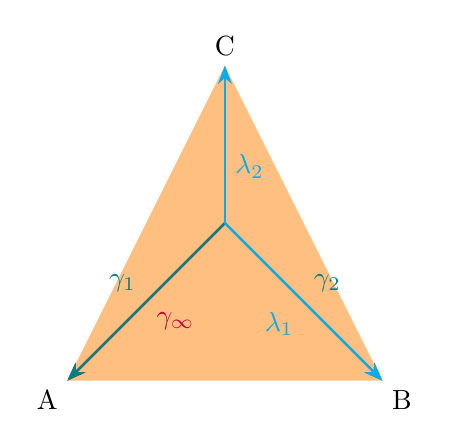
\begin{tikzpicture}[scale=2]
    % Define points for the convex hull
    \coordinate (A) at (-1,-1);
    \coordinate (B) at (1,-1);
    \coordinate (C) at (0,1);

    % Draw the convex hull
    \fill[orange!50] (A) -- (B) -- (C) -- cycle;

    % Draw the origin
    \coordinate (O) at (0,0);

    % Draw the gamma_infinity vector
    \draw[-Stealth, purple, thick] (O) -- node[midway, below right] {$\gamma_\infty$} (A);

    % Draw the lambda_r vectors
    \draw[-Stealth, teal, thick] (O) -- node[midway, above left] {$\gamma_1$} (A);
    \draw[-Stealth, teal, thick] (O) -- node[midway, above right] {$\gamma_2$} (B);
    \draw[-Stealth, cyan, thick] (O) -- node[midway, below left] {$\lambda_1$} (B);
    \draw[-Stealth, cyan, thick] (O) -- node[midway, below right] {$\lambda_2$} (C);

    % Add labels
    \node[below left] at (A) {A};
    \node[below right] at (B) {B};
    \node[above] at (C) {C};
\end{tikzpicture}

% Bottom Figure: Canonical-Scalar Theory
\begin{tikzpicture}[scale=2]
    % Define points for the scalar field
    \coordinate (S) at (0,0);
    \coordinate (S1) at (1,0);
    \coordinate (S2) at (0,1);
    \coordinate (